\chapter{Umsetzung}
\label{chapter:implementation}
    In diesem Kapitel wird die Umsetzung des System erläutert.
    Zunächst wird die zur Implementierung verwendete Software näher erläutert.
    Anschließend werden Front- und Backend kurz vorgestellt und mit dem Entwurf aus Kapitel \ref{chapter:design} verglichen.
    
    \section{Verwendete Software}
        
    
    \section{Frontend}
        Die Entwürfe für das Frontend wurden ohne große Änderungen umgesetzt.
        
        \begin{figure}
            \centering
            \begin{subfigure}{0.49\textwidth}
                \includegraphics[width=1.0\textwidth]{./implementation/images/MockUpsFrontend/frontendLogin.png}
            \end{subfigure}
            \begin{subfigure}{0.49\textwidth}
                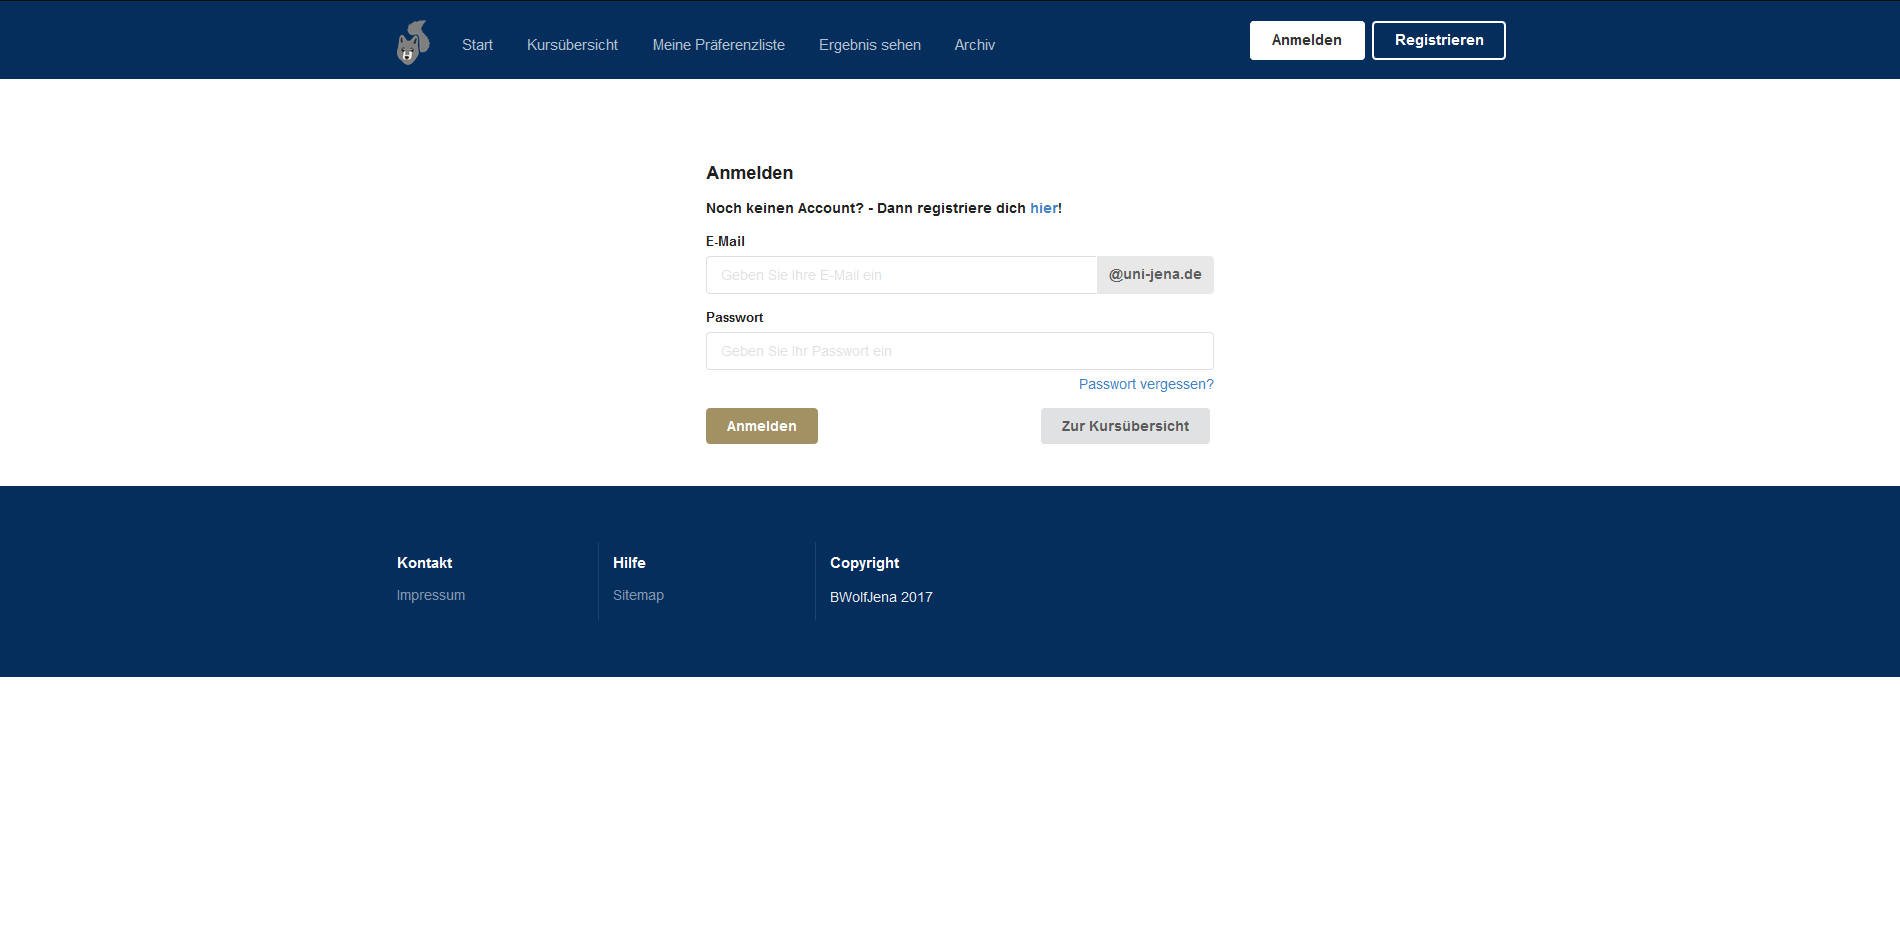
\includegraphics[width=1.0\textwidth]{./implementation/images/login.png}
            \end{subfigure}
            \caption{Gegenüberstellung von Entwurf der Login-Oberfläche (links) und Umsetzung (rechts)}
            \label{fig:comparisonLogin}
        \end{figure}
    
        In Abbildung \ref{fig:comparisonLogin} sind der Entwurf für die Login-Oberfläche und die Umsetzung selbiger gegenüber gestellt.
        Es fällt auf, dass die grobe Struktur der Seite bis auf kleine Änderungen mit dem Entwurf übereinstimmt.
        Unterschiede lassen sich vor allem in der Kopfzeile erkennen.
        So wurde der Reiter \textit{Start} hinzugefügt.
        Anders als zuvor angedacht, fiel die Entscheidung für eine Startseite, in der das Empiriepraktikum kurz vorgestellt wird.
        Des Weiteren wurde der Reiter \textit{Einschreiben} aus Gründen der Verständlichkeit in \textit{Meine Präferenzliste} umbenannt.
        Die Seite erfüllt jedoch die selbe Funktion.
    
        \begin{figure}
            \centering
            \begin{subfigure}{0.49\textwidth}
                \includegraphics[width=1.0\textwidth]{./implementation/images/MockUpsFrontend/frontendCourses.png}
            \end{subfigure}
            \begin{subfigure}{0.49\textwidth}
                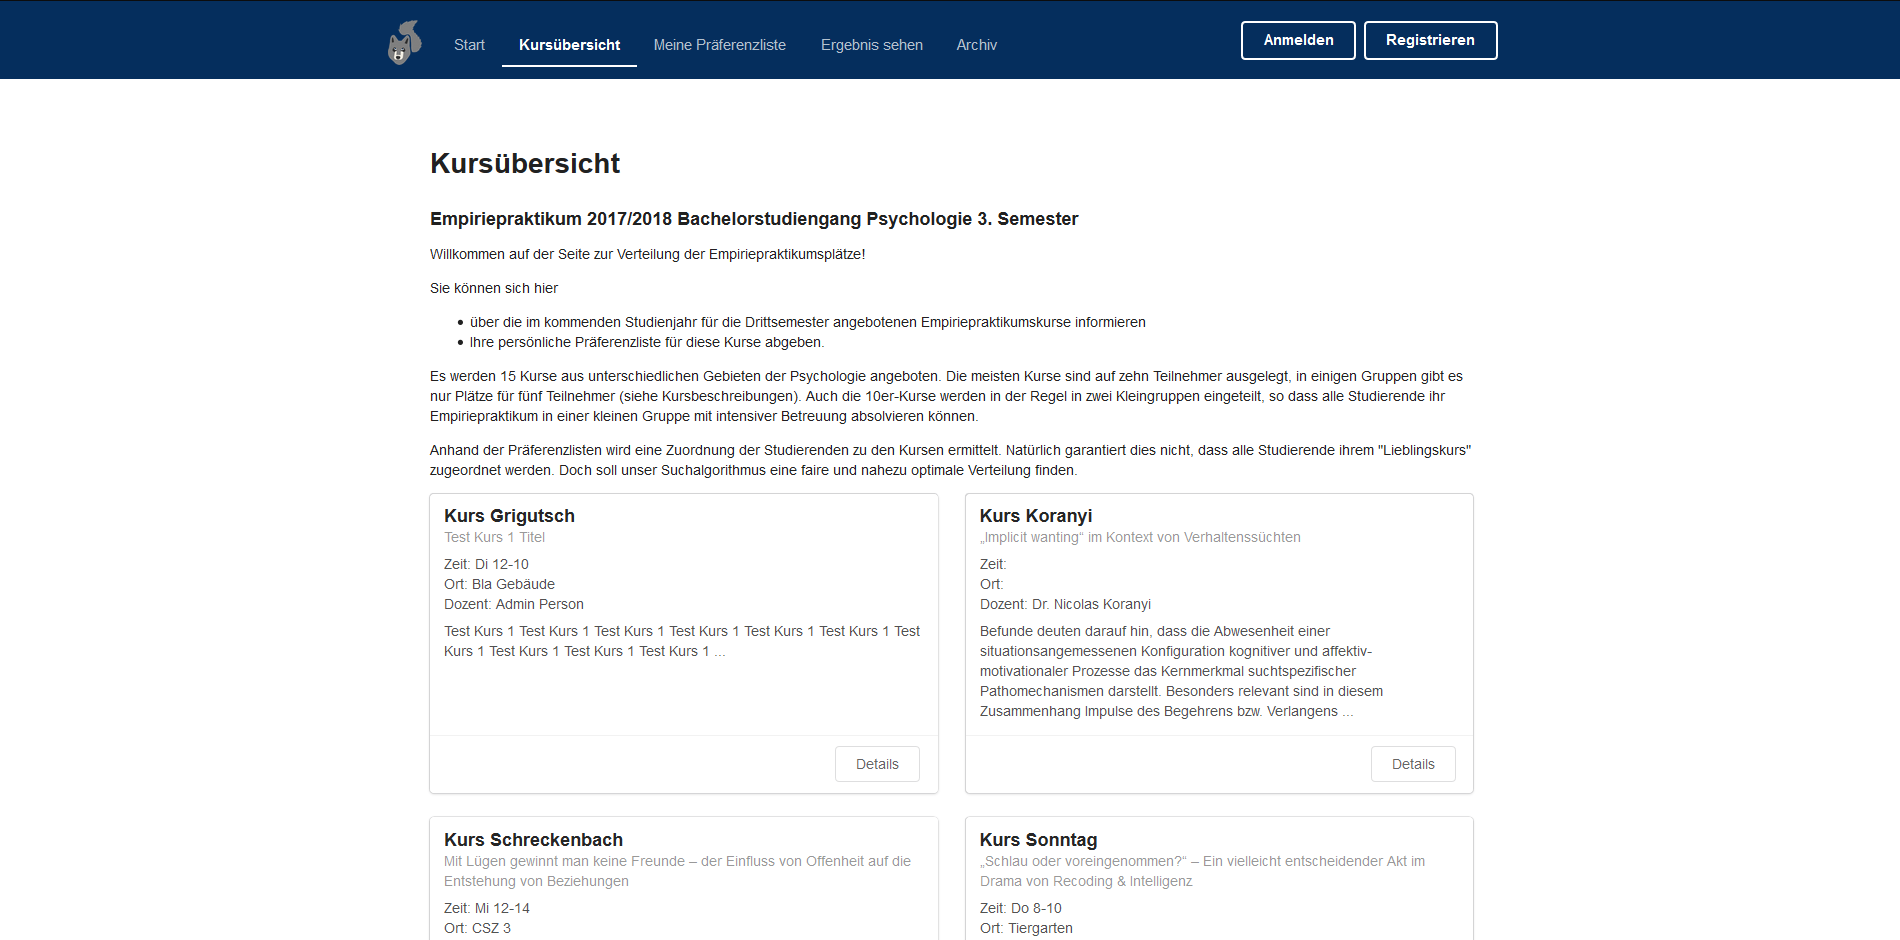
\includegraphics[width=1.0\textwidth]{./implementation/images/courses.png}
            \end{subfigure}
            \caption{Gegenüberstellung von Entwurf der Kursübersicht (links) und Umsetzung (rechts)}
            \label{fig:comparisonCourses}
        \end{figure}
    
        Abbildung \ref{fig:comparisonCourses} zeigt Entwurf und Umsetzung der Kursübersicht.
        Die Struktur des Entwurfs wurde direkt umgesetzt.
        Wie in Kapitel \ref{chapter:requirements} beschrieben, ist es, wie in Abbildung \ref{fig:comparisonCourses} zu sehen ist, möglich auch ohne eine Anmeldung auf die Kursübersicht zuzugreifen.
        Es ist anzumerken, dass die Fußleiste auch in der Kursübersicht wie in Abbildung \ref{fig:comparisonCourses} den Abschluss der Seite bildet und lediglich durch die Menge an Kursen nicht zu sehen ist.
        
        \begin{figure}
            \centering
            \begin{subfigure}{0.49\textwidth}
                \includegraphics[width=1.0\textwidth]{./implementation/images/MockUpsFrontend/frontendPreferences.png}
            \end{subfigure}
            \begin{subfigure}{0.49\textwidth}
                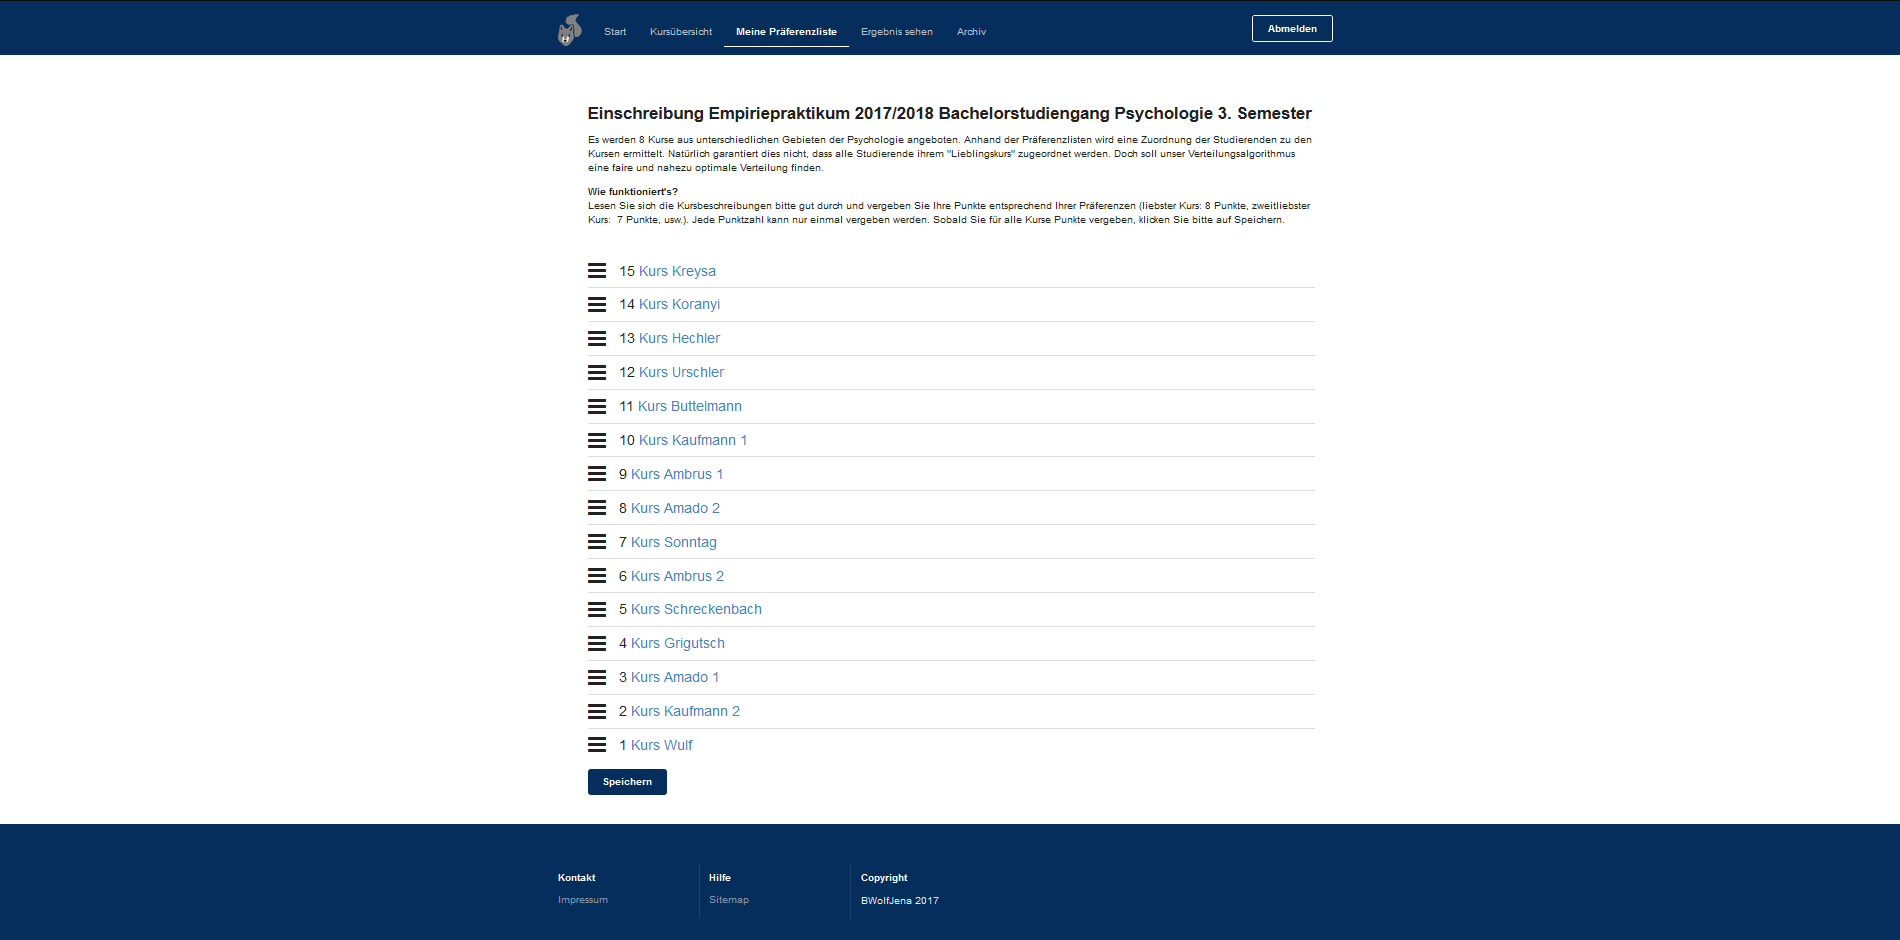
\includegraphics[width=1.0\textwidth]{./implementation/images/preferences.png}
            \end{subfigure}
            \caption{Gegenüberstellung von Entwurf der Einschreibungs-Oberfläche (links) und Umsetzung (rechts)}
            \label{fig:comparisonPrefenrences}
        \end{figure}
    
    
    \section{Backend}
    
        \begin{figure}
            \centering
            \begin{subfigure}{0.49\textwidth}
                \includegraphics[width=1.0\textwidth]{./implementation/images/MockUpsBackend/backendManageCourses.png}
            \end{subfigure}
            \begin{subfigure}{0.49\textwidth}
                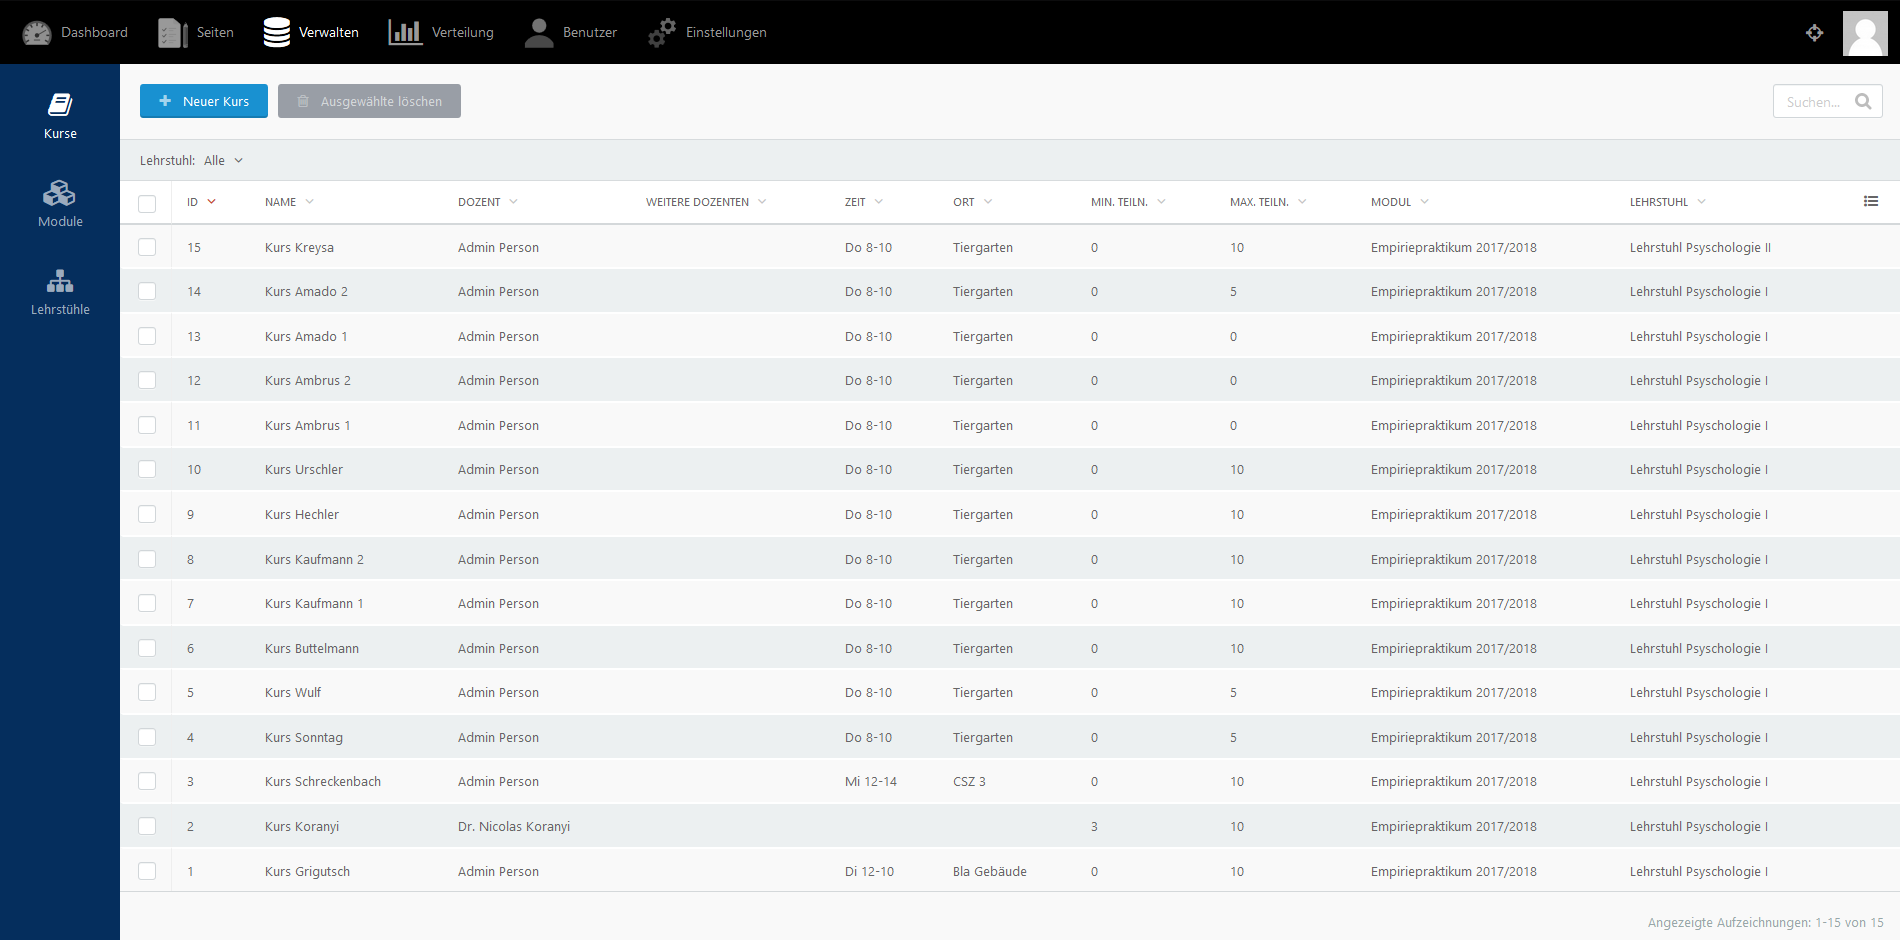
\includegraphics[width=1.0\textwidth]{./implementation/images/manageCourses.png}
            \end{subfigure}
            \caption{Gegenüberstellung von Entwurf der Kursverwaltung (links) und Umsetzung (rechts)}
            \label{fig:comparisonManageCourses}
        \end{figure}
        
        \begin{figure}
            \centering
            \begin{subfigure}{0.49\textwidth}
                \includegraphics[width=1.0\textwidth]{./implementation/images/MockUpsBackend/backendEdit.png}
            \end{subfigure}
            \begin{subfigure}{0.49\textwidth}
                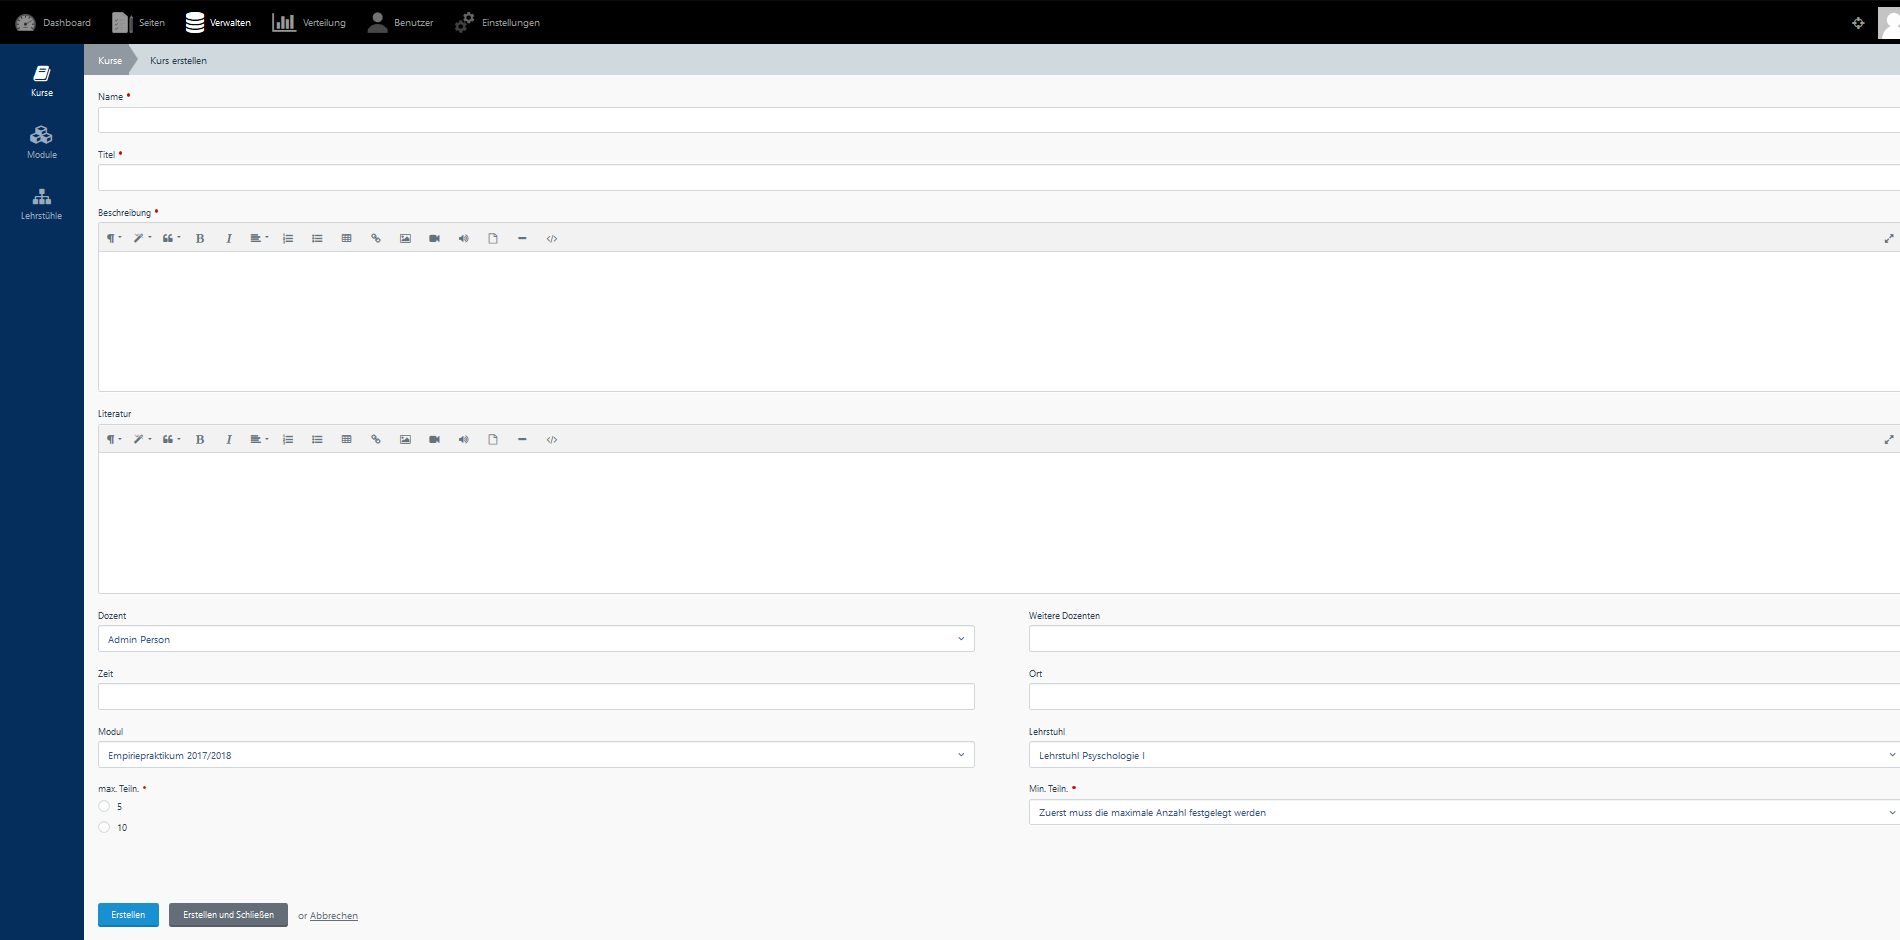
\includegraphics[width=1.0\textwidth]{./implementation/images/edit.png}
            \end{subfigure}
            \caption{Gegenüberstellung von Entwurf der Kurserstellung (links) und Umsetzung (rechts)}
            \label{fig:comparisonEdit}
        \end{figure}
    
        \begin{figure}
            \centering
            \begin{subfigure}{0.49\textwidth}
                \includegraphics[width=1.0\textwidth]{./implementation/images/MockUpsBackend/backendDistribution.png}
            \end{subfigure}
            \begin{subfigure}{0.49\textwidth}
                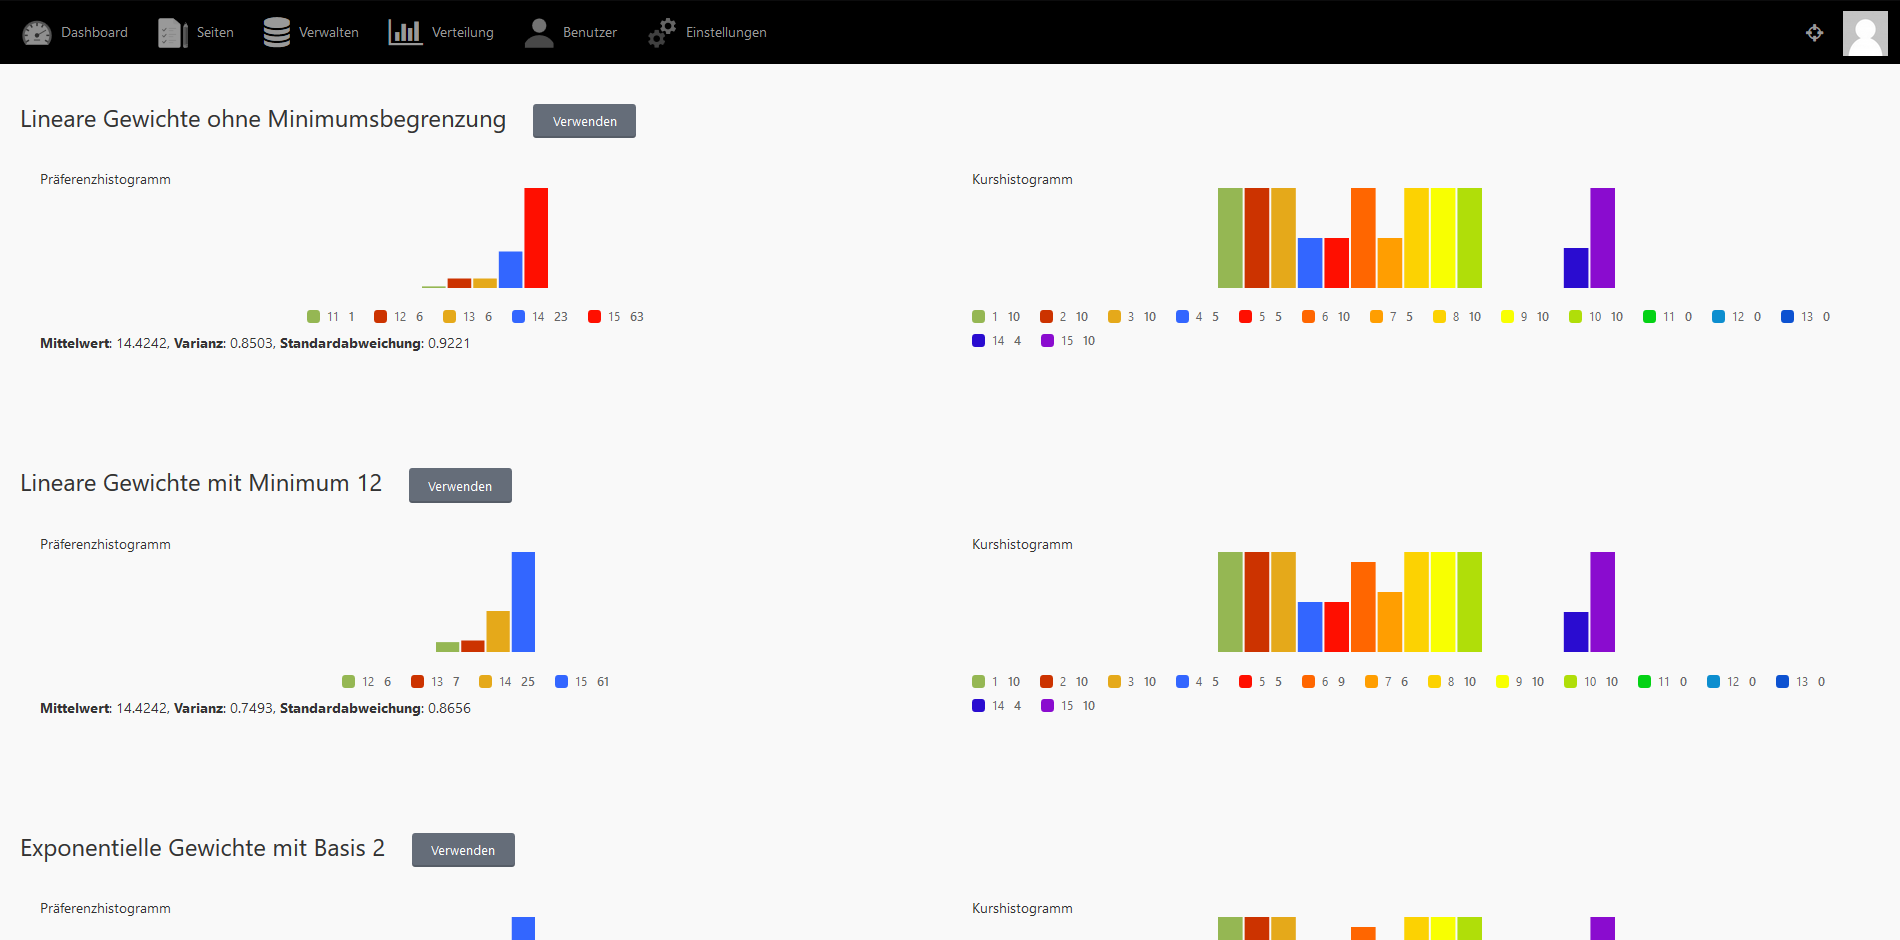
\includegraphics[width=1.0\textwidth]{./implementation/images/distribution.png}
            \end{subfigure}
            \caption{Gegenüberstellung von Entwurf der Anzeige der Verteilungsvorschläge (links) und Umsetzung (rechts)}
            \label{fig:comparisonDistribution}
        \end{figure}